\documentclass[aspectratio=169]{beamer}
\usepackage{goethecc}

\usepackage{color, colortbl}

\usepackage[USenglish]{babel}
\usepackage{amsmath,amsfonts,amssymb,textcomp}
\usepackage{graphicx}
\usepackage{pdfpages}


\usepackage{latexsym}
\usepackage{xspace}

\usepackage{aurical}

\usepackage{intcalc}

\usepackage{siunitx}
\input{turing}

\sisetup{locale = DE}

\usepackage{xstring}
\usepackage{tikz}
\usepackage{pgf}
\usepackage{mathtools,pgfplots}
\usetikzlibrary{calc}   
\usetikzlibrary{positioning}
\usetikzlibrary{automata}
\usetikzlibrary{arrows}   
\usepackage{soul}
\graphicspath{{./images/}}

%%%%%%%%%%%%%%%%%%%%%%%%%%%%%%%%%%%%%%%%%%%%
% We gonna write a lot of unary numbers; let TeX do the work for us
\newcommand{\unum}[1]{
	\ifthenelse{\equal{0}{#1}}{}{
	\ifthenelse{\equal{1}{#1}}{1}{%
	1%
	\foreach \unumj in {\intcalcDec{#1},...,1} {%
		\ifthenelse{\equal{\intcalcMod{\unumj}{3}}{0}}{\textquoteleft}{}%<-- this is the sep
		1%<-- this is the actual digit
	}%
}}}
\newcommand{\ttunum}[1]{\ensuremath{\mathtt{\unum{#1}}}}


%%%%%%%%%%%%%%%%%%%%%%%%%%%%%%%%%%%%%%%%%%%%
% General purpose tikz attributes for condition formating
\tikzset{onslide/.code args={<#1>#2}{%
    \only<#1>{\pgfkeysalso{#2}} % \pgfkeysalso doesn't change the path
}}
\tikzset{onslidep/.code args={<#1>#2}{%
		\ifthenelse{#1 = 0}{}{\only<#1->{\pgfkeysalso{#2}}} % \pgfkeysalso doesn't change the path
}}
\tikzset{onslidepp/.code args={<#1><#2>#3}{%
		\ifthenelse{#1=0 \OR #2=0}{}{\only<#1-#2>{\pgfkeysalso{#3}}} % \pgfkeysalso doesn't change the path
	}}
\tikzset{temporal/.code args={<#1>#2#3#4}{%
    \temporal<#1>{\pgfkeysalso{#2}}{\pgfkeysalso{#3}}{\pgfkeysalso{#4}} % \pgfkeysalso doesn't change the path
}}
\tikzset{onif/.code args={<#1>#2}{%
 	\ifthenelse{#1}{\pgfkeysalso{#2}}{}%
}}

\newcommand{\tikzanchor}[1]{\tikz[overlay, remember picture]{\node[anchor=text, inner sep=0] (#1) {\phantom{Ig}};}}


%%%%%%%%%%%%%%%%%%%%%%%%%%%%%%%%%%%%%%%%%%%%
% Formating of our Turing Machines 		
\def\cellSize{27pt}
\def\tmBlankSym{\ensuremath{\mathbb B}}
		
\tikzset{tmCell/.style={font={\Large\tt}, minimum height=\cellSize, minimum width=\cellSize}}
\tikzset{tmCellActive/.style={tmCell}}
\tikzset{tmCellBlank/.style={dunkelgrau!50, fill=sandgrau}}
\tikzset{tmHeadMarker/.style={circle, draw, ultra thick, emorot, minimum width=0.9*\cellSize, minimum height=0.9*\cellSize}}

\tikzset{tmState/.style={draw, minimum width=6em, rounded corners=0.4em}}
\tikzset{tmStateActive/.style={fill=emorot!50}}
\tikzset{tmTrans/.style={draw, ->, shorten >=2pt, thick, auto}}
\tikzset{tmTransActive/.style={emorot}}


\tikzset{loop above/.style={looseness=8, out=120, in=60}}
\tikzset{loop below/.style={looseness=8, out=300, in=240}}
 		

\begin{document}
\title{
	Und womit rechnest du so? \\[-0.5em]
	\textcolor{dunkelgrau}{\small \emph{mit Folien von Cyriax und Manuel}}
}
\author{
	Jonathan Cyriax Brast\\
	Manuel Penschuck \\
} 
\date{10. Juni 2017}

{
\setbeamertemplate{footline}{} 
\goethccBgTitel
\begin{frame}
  \titlepage
  \begin{tikzpicture}[overlay]
	  \node[anchor=south east, xshift=-0.08\textwidth, yshift=0.05\textheight, at=(current page.south east)] {
\includegraphics[width=0.15\textwidth]{cs.pdf}};
  \end{tikzpicture}
\end{frame}
}
\addtocounter{framenumber}{-1}


%\frame{\frametitle{Outline}\tableofcontents}

%%%%%%%%%%%%%

\input{intro}
\begin{frame}{}
	\begin{center}
		\scalebox{1.5}{\Huge \textcolor{emorot}{Subtraktion}}
		
		\vspace{1em}
		
		{\large \textcolor{goetheblau}{Minus-Rechnen}}
	\end{center}
\end{frame}


\begin{frame}{Subtraktion}
	\begin{center}
		\Huge

		\only<+>{
			\scalebox{1.5}{\Huge \textcolor{emorot}{Selbsttest}}
		}		
		\only<+>{$\textcolor{goetheblau}{7}-\textcolor{emorot}{3}=\underline{\phantom4}$}
		\only<+>{$\textcolor{goetheblau}{7}-\textcolor{emorot}{3}=\textcolor{orange}{\underline{4}}$}
		
		\only<+>{
			\scalebox{1.5}{\Huge \textcolor{emorot}{Und noch einer \ldots}}
		}		
		\only<+>{$\textcolor{goetheblau}{123}-\textcolor{emorot}{45}=\underline{\phantom{78}}$}
		\only<+>{
			$\textcolor{goetheblau}{123}-\textcolor{emorot}{45}=\textcolor{orange}{\underline{78}}$
			\begin{tikzpicture}[overlay, remember picture]
				\node[at=(current page.south east), anchor=south east, xshift=-2em, yshift=2em]  {\Large \color{sandgrau} \#NotMyPisa};
			\end{tikzpicture}
		}
	\end{center}
\end{frame}

\begin{frame}{Unäre Zahlen -- römisch für Arme}
	\begin{tikzpicture}[remember picture, overlay]
	\node[at=(current page.north), yshift=-3em, anchor=north, draw, fill=sandgrau, minimum width=2\textwidth, minimum height=2.5em] {
		\large
		Wir stellen die \textcolor{goetheblau}{Zahl $x$} durch  \textcolor{emorot}{$x$ Einsen} dar.
	};
	\end{tikzpicture}


	\begin{center}
		\begin{tikzpicture}[
			node distance=0,
			dnum/.style={align=right, text width=2em},
			unum/.style={align=right, text width=8em}
		]
			\node (a0) {};
			\foreach \i in {1, ..., 5} {
				\node[dnum, below=of a\intcalcDec\i] (a\i) {$\textcolor{goetheblau}{\i}_\text{Dez}$};
				\node[right=of a\i] (b\i) {$=$};
				\node[unum, right=of b\i] (c\i) {$\textcolor{emorot}{\ttunum{\i}}_\text{Unär}$};
	
				\node[dnum, right=2em of c\i] (d\i) {$\textcolor{goetheblau}{\intcalcAdd5\i}_\text{Dez}$};
				\node[right=of d\i] (e\i) {$=$};
				\node[unum, right=of e\i] (f\i) {$\textcolor{emorot}{\ttunum{\intcalcAdd5\i}}_\text{Unär}$};
			}
		\end{tikzpicture}
	\end{center}
\end{frame}

\begin{frame}{Wie beschreiben wir unäre Subtraktion?}
	\vspace{4.5em}

	\begin{center}
		\scalebox{1.3}{
			\begin{tikzpicture}[
				number/.style={text width=3.8em, align=right, anchor=north west, inner sep=0.1em, minimum height=1.5em, orange},
				header/.style={number, font={\bf}}
			]
				\def\sx{4em}
				\def\sy{1.5em}
	
				\node[fill=sandgrau, anchor=north west, minimum width=7*\sx, minimum height=\sy, inner sep=0] at (0,0)  {};
				\node[fill=sandgrau, anchor=north west, minimum width=\sx, minimum height=11em, inner sep=0] at (0,0)  {};
			
				\foreach \x in {1, ..., 5} {
					\node[header, goetheblau] at (\x*\sx, 0) {$\mathbf{\unum{\x}}$};
					\node[header, emorot] at (0, -\x*\sy) {$\mathbf{\unum{\x}}$};
	
					\node[header, goetheblau] at (6*\sx, 0) {$\cdots$};
					\node[header, emorot, minimum height=2em] at (0, -6*\sy) {$\vdots$\ \ \phantom.};
	
					\node[number, fill=sandgrau] at (6*\sx, -\x*\sy) {$\cdots$};
					\node[number, fill=sandgrau, minimum height=2em] at (\x*\sx, -6*\sy) {$\vdots$};
	
					
					\foreach \y in {1, ..., 5} {
						\ifthenelse{\equal{\intcalcCmp\x\y}{-1}}{
							\node[number, fill=sandgrau] at (\x*\sx, -\y*\sy) {};
						}{
							\node[number] at (\x*\sx, -\y*\sy) {
								\ifthenelse{\equal\x\y}{\textcolor{emorot}{\only<2>{0}}} 
								{\ttunum{\intcalcSub\x\y}}
							};
						}
					}
				}
				
				\node[header, fill=sandgrau, minimum height=2em] at (6*\sx, -6*\sy) {$\ddots$};
				
				\node[goetheblau, draw, minimum width=28em, minimum height=11em, anchor=north west, onslide={<4->white, fill=white, opacity=0.8}] (tabborder) {};
			\end{tikzpicture}
		}
	\end{center}

	\begin{tikzpicture}[remember picture, overlay]
		\node[at=(current page.north), yshift=-3em, anchor=north, draw, fill=sandgrau, minimum width=2\textwidth, minimum height=2.5em] {
			\Huge
			$\textcolor{goetheblau}{a} - \textcolor{emorot}{b} = \textcolor{orange}{c}$
		};
		
		\only<4->{
			\node[draw, radius=0.5em, rounded corners=1em, emorot, fill=white, opacity=0.8, inner sep=2em] at (current page) {\phantom{\Huge Nicht praktikabel für große Zahlen!}};
			
			\node[emorot, inner sep=2em] at (current page) {\Huge Unpraktisch für große Zahlen!};
		}
	\end{tikzpicture}
\end{frame}

\newcommand{\removeDigit}[1]{%
	\only<-\intcalcDec{#1}>{1}%
	\only<#1>{\textcolor{emorot}{\underline 1}}%
}

\begin{frame}{Wir brauchen einen Algorithmus}
	\begin{tikzpicture}[remember picture, overlay]
	\node[at=(current page.north), yshift=-3em, anchor=north, draw, fill=sandgrau, minimum width=2\textwidth] {
		\Huge
		$\textcolor{goetheblau}{a} - \textcolor{emorot}{b} = \textcolor{orange}{c}$
	};
	\end{tikzpicture}
	
	\begin{columns}[t]
		\begin{column}{0.7\textwidth}
			\Large
			\setbeamertemplate{enumerate items}[default]
			\begin{enumerate}
				\item
					\tikzanchor{step1}%
					\textbf{Wenn} \textcolor{emorot}{$b$} keine Ziffer mehr hat,\\
					\tikzanchor{step1a}
					\textbf{dann} \textcolor{orange}{\textbf{antworte} $c \gets a$} und \textbf{halte}
					
					\vspace{1em}

				
				\item
					\tikzanchor{step2}%
					\texttt{Entferne} letzte Ziffer von \textcolor{goetheblau}{a}\\
					\texttt{Entferne} letzte eine Ziffer von \textcolor{emorot}{b}

					\vspace{1em}

				
				\item 
					\tikzanchor{step3}%
					\textbf{Springe} zu \textcolor{goetheblau}{1.}
			\end{enumerate}
		\end{column}%
		
		\begin{column}{0.25\textwidth}
			\Huge

			$\textcolor{goetheblau}{a}$: \hfill 1\removeDigit6\removeDigit3\\
			$\textcolor{emorot}{b}$: \hfill \removeDigit6\removeDigit3\\
			$\textcolor{orange}{c}$: \hfill \only<-8>{?}\only<9>{\textcolor{emorot}{1}}
			
			\uncover<9>{\begin{center}
					Halt, Stop!
			\end{center}}
			
		\end{column}
	\end{columns}
	
	\begin{tikzpicture}[
		overlay, remember picture,
		prog counter/.style={emorot, <-, ultra thick}
	]
		\path[prog counter, onslide={<2,5,8>draw}] ($(step1)+(-2.5em,0)$) to ++(-2em, 0);
		\path[prog counter, onslide={<9>draw}]     ($(step1a)+(-2.5em,0)$) to ++(-2em, 0);		
		\path[prog counter, onslide={<3,6>draw}]   ($(step2)+(-2.5em,0)$) to ++(-2em, 0);
		\path[prog counter, onslide={<4,7>draw}]   ($(step3)+(-2.5em,0)$) to ++(-2em, 0);
	
	\end{tikzpicture}
	
\end{frame}


\newcommand{\handwrittenNoteBelow}[3]{
	\node[goetheblau, anchor=west, align=left] at ($(#1)+(1.6,-0.6)#3$) {\Large \Fontauri\bfseries #2};
	\path[<-, draw, goetheblau, ultra thick, bend right=15] ($(#1)#3$) to ++(1.5,-0.5);
}

\newcommand{\handwrittenNoteAbove}[3]{
	\node[goetheblau, anchor=west, align=left] at ($(#1)+(1.6,0.6)#3$) {\Large \Fontauri\bfseries #2};
	\path[<-, draw, goetheblau, ultra thick, bend left=15] ($(#1)#3$) to ++(1.5,0.5);
}


\begin{frame}{}
	\begin{center}
		\Huge
		\only<1>{Turing Maschine}
		\only<2-3>{%
			\only<2>{\includegraphics[height=0.6\textheight]{images/cumberbatch.jpg}}%
			\only<3>{\includegraphics[height=0.6\textheight]{images/turing.jpg}}%
			\hspace{2em}
			\includegraphics[height=0.6\textheight]{images/nos2012.jpg}
			\vspace{1em}
						
			Alan M. Turing\\
			1912 -- 1954 
		}
		\only<4>{
			\fbox{\includegraphics[height=0.6\textheight]{images/turing1936.png}}
			\vspace{1em}
			
			\textquotedblleft On Computable Numbers, With an Application to the Entscheidungsproblem\textquotedblright\\
			\textcolor{goetheblau}{[A. Turing, 1936/37]}
		}
	\end{center}
\end{frame}


\begin{frame}{Turing Maschine}
	\begin{center}
		\vspace{2em}

		\uncover<7->{
			\begin{tikzpicture}[remember picture]
				\node[tmState, draw] (stateA) {Zustand A};
				\node[tmState, draw, anchor=west] (stateB) at ($(stateA.east) + (5,0)$)  {Zustand B};
				
				\path[draw, ->, thick, bend left=10, shorten >=5pt, onslide={<8>, emorot}] (stateA) to node[above] {\tikzanchor{transAnchor} \texttt 0 zu \texttt 1, $\Rightarrow$} (stateB);
				\path[draw, ->, thick, bend left=10, shorten >=5pt] (stateB) to node[below,align=left] {\texttt 0 zu \texttt 0, $\Leftarrow$ \\ \texttt 1 zu \texttt 1, $\Leftarrow$} (stateA);
			\end{tikzpicture}

			\begin{tikzpicture}[remember picture, overlay]
				\handwrittenNoteBelow{stateB}{Programm}{-(2,1)}
							
			
				\only<8->{
					\handwrittenNoteAbove{transAnchor}
					{\normalfont\normalsize Wenn \textcolor{emorot}{\texttt 0} gelesen:\\ Schreibe \textcolor{emorot}{\texttt 1}, Kopf nach rechts}
					{+(1.8,0.2)}
				}
			\end{tikzpicture}			
		}

		\vspace{3em}
		
		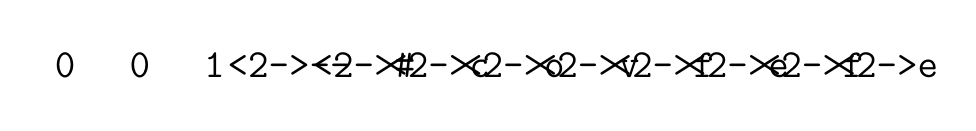
\begin{tikzpicture}[
			remember picture
		]
			\node[tmCell                ] (tmbandcell0) {};		

			\foreach \x  [count=\i] in {
				0,0,1,
				\only<2->{--},
				\only<2->{\#},
				\only<2->{c},
				\only<2->{o},
				\only<2->{v},
				\only<2->{f},
				\only<2->{e},
				\only<2->{f},
				\only<2->{e}
			} {
				\node[tmCell] at ($(tmbandcell0) + (\i*\cellSize,0) - (\cellSize,0)$) {\x};
			}
		\end{tikzpicture}
			

		\begin{tikzpicture}[overlay, remember picture]
			\only<1-2> {
				\handwrittenNoteBelow{tmbandcell0}{Eingabe}{+(2, -0.6)}
			}
		
			\only<1> {\tmDrawGrid{0}{3}}
			\only<2> {\tmDrawGrid{0}{12}}
			\only<3-> {
				\foreach \i in {1,...,5} {
					\node[tmCell, tmCellBlank] at ($(tmbandcell0) - (\i*\cellSize,0)$) {\only<4->{\tmBlankSym}};
					\node[tmCell, tmCellBlank] at ($(tmbandcell0) + (\i*\cellSize,0) + (11*\cellSize, 0)$) {\only<4->{\tmBlankSym}};
				}
				\tmDrawGrid{-5}{18}

				\handwrittenNoteBelow{tmbandcell0}{Speicher / Band}{+(2, -0.6)}
			}
			
			\only<5->{
				\node[tmHeadMarker, at=(tmbandcell0)] {};
				\handwrittenNoteAbove{tmbandcell0}{Kopf}{+(0.4, 0.4)}
			}
			
			\only<6->{
				\node[emorot, anchor=north, at=(tmbandcell0.south), yshift=-0.2em] {\Large $\Leftarrow, \Downarrow, \Rightarrow$};
			
			}
		\end{tikzpicture}
	\end{center}
\end{frame}
\def\turingAStateDef{
%%%%%% BEGIN-TM: turingI, B111-11B %%%%%
	\tmstate{firstMinus}{Suche Minus}  {}{}
	\tmstate{rightDigit}{Rechte Ziffer}{above right=of firstMinus}{}
	\tmstate{leftDigit} {Linke Ziffer} {below right=of firstMinus}{}
	\tmstate{cleanUp}   {Aufräumen}    {below right=of rightDigit}{}
	
	\tmstart{firstMinus}
	
	\tmtrans{firstMinus}{firstMinus}{\trans 11R }{loop below}{}
	\tmtrans{firstMinus.east}{rightDigit.west}{\trans --R}{above,sloped}{}
	
	\tmtrans{rightDigit}{rightDigit}{\trans --R}{loop above}{}
	\tmtrans{rightDigit}{leftDigit}{\trans 1-L}{bend right, below, left}{}
	\tmtrans{rightDigit.east}{cleanUp.west}{\trans BBL}{above, sloped}{}
	
	
	\tmtrans{leftDigit}{leftDigit}{\trans --L}{loop below}{}
	\tmtrans{leftDigit}{rightDigit}{\trans 1-R}{bend right, below, right}{}
	
	\tmtrans{cleanUp}{cleanUp}{\trans -BL}{loop below}{}
%%%%%% END-TM: turingI %%%%%
}

\newcommand{\tmADraw}[1]{
	\newcommand{\tmStateCurrent}{#1}

	\begin{center}
		\scalebox{0.9}{
			\tmDrawStates{\turingAStateDef}
		}
		
		\vspace{2em}
		
		\tmDrawBand
	\end{center}
	
	\begin{tikzpicture}[remember picture, overlay]
		\foreach \i in {1,...,10} {
			\node[tmCell, tmCellBlank] at ($(tmbandcell0) - (\i*\cellSize,0) + (\cellSize, 0)$) {\tmBlankSym};
			\node[tmCell, tmCellBlank] at ($(tmbandcell0) + (\i*\cellSize,0) + (\thetmBandCnt*\cellSize, 0)$) {\tmBlankSym};
		}
		
		\tmDrawGrid{-10}{20}
	\end{tikzpicture}
}


\newcommand{\tmACallback}[1]{\only<+>{\tmADraw{#1}}}
\tmSetup{A}{\turingAStateDef}

\begin{frame}{Subtraktion: $3 - 2 = ?$}
	\tmExecute{A}{111-11B}{\tmACallback}
\end{frame}

\newcommand{\bsl}{\textbackslash}

\begin{frame}{sed - h\"a, was?}
	sed steht f\"ur Stream Editor\\
	also:\\
	sed nimmt sich einen Textstrom und pfuscht in dem irgendwie rum:\\
	Beispiel:\\
	\texttt{s/2016/2017/} = Suche 2016 und ersetze es mit 2017\\
	''NoS Vortrag 2016'' $\rightarrow$ ''NoS Vortrag 2017''\\
\end{frame}


%TODO: braucht noch: wenn ich nichts finde passiert nichts...
\begin{frame}{Editwar mit sed}
	''Manu ist der Beste!''\\
	\quad\quad\texttt{s/der Beste/doof/}\\
	''Manu ist doof!''\\
	\quad\quad\texttt{s/Manu/Cyriax/}\\
	''Cyriax ist doof!''\\
	\quad\quad\texttt{s/ist doof/hat Manus Vortrag gekapert/}\\
	''Cyriax hat Manus Vortrag gekapert!''\\
	\quad\quad\texttt{s/(.*) hat (.*)s Vortrag gekapert/\bsl2 hat \bsl1s Vortrag gekapert/}\\
	''Manu hat Cyriaxs Vortrag gekapert!''
	\quad\quad\texttt{s/(.*) hat (.*)s Vortrag gekapert/\bsl2 hat \bsl1s Vortrag gekapert/}\\
	''Cyriax hat Manus Vortrag gekapert!''
\end{frame}

\begin{frame}{Turingmaschine Idee}
	Wir brauchen also:\\
	1. Zustand\\
	2. Zustands\"uberg\"ange\\
	2. Band\\
	3. Kopf\\
\end{frame}

\begin{frame}{Turingmaschine Zust\"ande}
	%TODO tikz Bild NeuerZustand0 <-0A- AlterZustand -1B-> NeuerZustand1
	Wir merken uns den Zustand und den Rest vom Wort:\\
	''ZUSTAND:X''\\
	Jeder \"Ubergang ist ein Suchen und Ersetzen:\\
	\texttt{s/AlterZustand:0/NeuerZustand0:A/}\\
	\texttt{s/AlterZustand:1/NeuerZustand1:B/}
\end{frame}

\begin{frame}{Turingmaschine BandKopfApparat}
	%\begin{dummeIdee}
	@ sieht aus wie ein Kopf...\\
	%\end{dummeIdee}
	Nach links gehen:\\
	''Hallo W@elt'' $\rightarrow$ ''Hallo @Welt''\\
	\texttt{s/(.*)(.)@(.*)/\bsl1@\bsl2\bsl3/}\\
	e lesen und \"a schreiben:\\
	''Hallo W@elt'' $\rightarrow$ ''Hallo W@\"alt''\\
	\texttt{s/(.*)@e(.*)/\bsl1@\"a\bsl2/}\\
	Beides Zusammen:
	''Hallo W@elt'' $\rightarrow$ ''Hallo @W\"alt''\\
	\texttt{s/(.*)(.)@e(.*)/\bsl1@\bsl2\"a\bsl3/}\\


\end{frame}






\end{document}

